\begin{figure}[h]
    \centering
    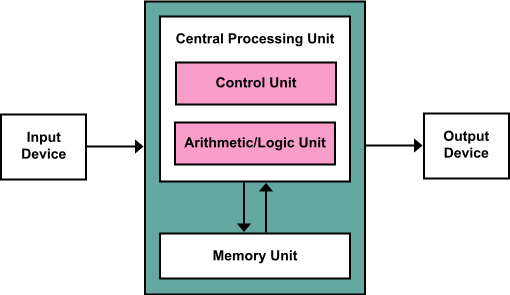
\includegraphics[scale=0.5]{CPUBASICDIAG}
    \caption{Diagram Sederhana CPU}
    \label{fig:CPUBASICDIAG}
\end{figure}

Cara kerja suatu CPU dapat digambarkan secara sederhana sepeti di Gambar\ref{fig:CPUBASICDIAG}.
Di diagram tersebut dapat dilihat ada tiga Unit Dasar CPU yang bertugas untuk melakukan
kalkulasi-kalkulasi penting bagi komputer.

Secara tingkatan, sebuah Control Unit adalah Unit terpenting, karena ialah yang mengatur
unit-unit lain yang dibawahnya, kemudian diikuti oleh Unit Arithmetic-Logic yang
adalah bagian dimana semua perhitungan aritmatika dan logika terjadi, dan terakhir
adalah Memory Unit, yang mempercepat kerja kedua unit yang lain tersebut, karena
di unit ini CPU bisa dapat media penyimpanan yang berkecepatan tinggi.

Suatu CPU ketika berkerja, akan menerima instruksi dari program-program yang menyala
di komputer, dan kemudian memproses instruksi tersebut menggunakan ketiga unit yang
telah disebut itu dan kemudian akan meng-outputkan nilai atau hasil sesuai dengan
instruksi.
